
\section*{Fluid-Structure Interaction between an elastic object and laminar incompressible flow}
The goal of this benchmark is to test the fluid and solid solver first separately and then together as a full FSI problem \cite{Hron2006a}. This benchmark is based on the older benchmark \" flow around cylinder\" with fluid considered incompressible and in the laminar regime, and the structure deformations are significant. The problem is setup with the solid submerged in the fluid, so that oscillations in the fluid deform the structure. We will measure the drag and lift around the circle and bar, and measure structural displacement at a given point. 

\subsection*{Problem Defintion}
\subsubsection*{Domain}
\begin{center}
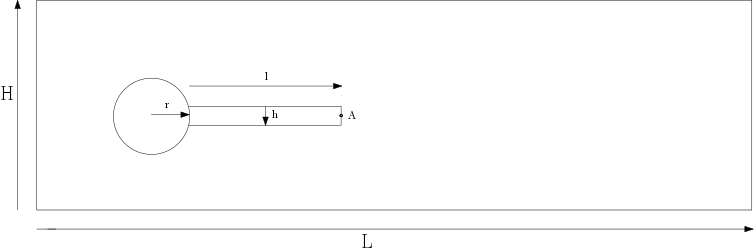
\includegraphics[scale=0.4]{./Verification_Validation/Hron_Turek/Domain_drawing.png}
\end{center}
The computational domain consists of a circle with an elastic bar behind the circle. The circle is positioned at (0.2, 0.2) making it 0.05 of center from bottom to top, this is done to induce oscillations to an otherwise laminar flow. 
This gives a force to the elastic bar. The parameters of the domain are:\\
L = 2.5, H = 0.41, l = 0.35, h = 0.02, A = (0.2,0.6) \\

\subsubsection*{Boundary conditions}
The fluid velocity has a parabolic profile on the inlet that changes over time:\\

\begin{align*}
u(0,y) &= 1.5u_0 \frac{y(H-y)}{(\frac{H}{2})^2}  \\
u(0,y,t) &= u(0,y)\frac{1-cos(\frac{\pi}{2}t)}{2} \text{  for  } t<2.0 \\
u(0,y,t) &= u(0,y) \text{  for  } t \leq 2.0
\end{align*}

We set no slip on the "floor" and "ceiling" so to speak.\\
$$ u(x,y,t) = 0 \text{  on  }  $$
On the fluid solid interface the boundary conditions are set to:
$$  \sigma_f n_f = \sigma_s n_s \hspace{4mm} on  \hspace{2mm}\Gamma^0 (interface)   $$
In our variational form we leave this out and so implying that they are equal.

\subsubsection*{Quantities for comparison}
When the fluid moves around the circle and bar it exerts a force. These are split into drag and lift and calculated as follows:
$$ (F_d, F_L) = \int_S \sigma_f n dS $$ 
where S is the part of the circle and bar in contact with the fluid. \\
We set a point A on the right side of the bar. This point is used to track the deformation in CSM and FSI tests. \\
In each test the numbers with ref are the values taken from the benchmark paper \cite{Hron2006a}
We integrate the mapped fluid stress tensor over the bar and circle and appended to lists: 
\begin{lstlisting}[language=Python]
Dr = -assemble((sigma_f_new(v,p,d,mu_f)*n)[0]*ds(6))
Li = -assemble((sigma_f_new(v,p,d,mu_f)*n)[1]*ds(6))
Dr += -assemble((sigma_f_new(v("-"),p("-"),d("-"),mu_f)*n("-"))[0]*dS(5))
Li += -assemble((sigma_f_new(v("-"),p("-"),d("-"),mu_f)*n("-"))[1]*dS(5))
Drag_list.append(Dr)
Lift_list.append(Li)
\end{lstlisting}
The deformation is calculated on the point A, and also added to lists:
\begin{lstlisting}[language=Python]
dsx = d(coord)[0]
dsy = d(coord)[1]
dis_x.append(dsx)
dis_y.append(dsy)
\end{lstlisting}
\subsection{Results}
\subsubsection*{CFD test}
The first two CFD tests are run with Reynolds number 20 and 100 giving steady drag and lift around the circle. CFD 3 has a Reynolds number 200 which will induce oscillations behind the circle, giving fluctuations in the drag and lift.
The CFD tests were run using the the bar as rigid object, that is the domain calculated is just the fluid domain. It is possible to also calculate with the bar and setting $\rho_s$ and $\mu_s$ to a large value. 

\begin{table}[h!]
\centering
\caption{CFD parameters}
\label{my-label}
\begin{tabular}{|l|l|l|l|}
\hline
Parameters & CFD1 & CFD2 & CFD3 \\ \hline
$\rho_f [10^3 \frac{kg}{m^3}]$ & 1 & 1 & 1 \\ \hline
$\nu_f [10^{-3} \frac{m^2}{s}]$ & 1 & 1 & 1 \\ \hline
$ U [\frac{m}{s}] $ & 0.2 & 1 & 2 \\ \hline
Re = $\frac{Ud}{\nu_f}$ & 20 & 100 & 200 \\ \hline
\end{tabular}
\end{table}

\begin{table}[h!]
\centering
\caption{CFD 1}
\label{my-label}
\begin{tabular}{|l|l|l|l|}
\hline
\textbf{elements} & \textbf{dofs} & \textbf{Drag} & \textbf{Lift} \\ \hline
6616 & 32472 & 14.2439 & 1.0869 \\ \hline
26464 & 124488 & 14.2646 & 1.11085 \\ \hline
105856 & 487152 & 14.2755 & 1.11795 \\ \hline
\textbf{ref} & \textbf{} & \textbf{14.29} & \textbf{1.119} \\ \hline
\end{tabular}
\end{table}

\begin{table}[h!]
\centering
\caption{CFD 2}
\label{my-label}
\begin{tabular}{|l|l|l|l|}
\hline
\textbf{elements} & \textbf{dofs} & \textbf{Drag} & \textbf{Lift} \\ \hline
6616 & 32472 & 135.465 & 6.27158 \\ \hline
26464 & 124488 & 136.566 & 9.82166 \\ \hline
105856 & 487152 & 136.573 & 10.4441 \\ \hline
\textbf{ref} & \textbf{} & \textbf{136.7} & \textbf{10.53} \\ \hline
\end{tabular}
\end{table}

\subsubsection*{CSM test}
The CSM test are calculated using only the bare and adding a gravity term $g$ with the same value but changing the parameters of solid.
As with the CFD test the first to CSM test cause a steady state solution, and CSM 3 is more slender causing the bar to go up and down in time. Our quantity for comparing there will be the deformation of the point $A$. In CSM 3 the energy is conserved by using a Crank-Nicholson scheme as can be seen in the plots fig7 (hvordan citer man et plot?)

\begin{table}[h!]
\centering
\caption{Parameters}
\label{my-label}
\begin{tabular}{|l|l|l|l|}
\hline
Parameters & CSM1 & CSM2 & CSM3 \\ \hline
$\rho_f[10^3 \frac{kg}{m^3}]$ & 1 & 1 & 1 \\ \hline
$\nu_f [10^{-3} \frac{m^2}{s}]$ & 1 & 1 & 1 \\ \hline
$u_0$ & 0 & 0 & 0 \\ \hline
$\rho_s[10^3 \frac{kg}{m^3}]$ & 1 & 1 & 1 \\ \hline
$\nu_s$ & 0.4 & 0.4 & 0.4 \\ \hline
$\mu_s[10^6 \frac{m^2}{s}]$ & 0.5 & 2.0 & 0.5 \\ \hline
$g $ & 2 & 2 & 2 \\ \hline
\end{tabular}
\end{table}

\begin{table}[h!]
\centering
\caption{CSM 1}
\label{my-label}
\begin{tabular}{|l|l|l|l|}
\hline
elements & dofs & ux $[10^{?3}]$ & uy $[10^{?3}]$ \\ \hline
725 & 1756 & -5.80951654915 & -59.4781430115 \\ \hline
2900 & 6408 & -6.77960453995 & -64.2130757639 \\ \hline
11600 & 24412 & -7.08597041285 & -65.635825349 \\ \hline
46400 & 95220 & -7.11626976966 & -65.7456687273 \\ \hline
ref & ref & -7.187 & -66.10 \\ \hline
\end{tabular}
\end{table}

% Please add the following required packages to your document preamble:
% \usepackage{booktabs}
\begin{table}[h!]
\centering
\caption{CSM 2}
\label{my-label}
\begin{tabular}{@{}|l|l|l|l|@{}}
\hline
Elements & Dofs & ux $[10^{-3}] $& ux $[10^{-3}] $\\ \hline
725 &  1756 & -0.375962146908 & -15.1950342598 \\ \hline
2900 & 6408 & -0.441308781709 & -16.4643196042\\ \hline
11600 & 24412 & -0.462087305294 & -16.8478689583 \\ \hline
46400 & 95220 & -0.464128022327 & -16.8782135872\\ \hline
ref & ref & -0.4690 & -16.97 \\ \hline
\end{tabular}
\end{table}

\begin{table}[h!]
\centering
\caption{CSM 3}
\label{my-label}
\begin{tabular}{|l|l|l|l|}
\hline
elements & dofs & ux $[10^3]$ & uy $[10^3]$ \\ \hline
725 & 1756 & $-11.743 \pm 11.744$ & $-57.952 \pm 58.940$ \\ \hline
2900 & 6408 & $-13.558 \pm 13.559$ & $ -61.968 \pm  63.440 $ \\ \hline
11600 & 24412 & $ -14.128 \pm 14.127$ & $-63.216 \pm 64.744 $ \\ \hline
46400 & 95220 & $ -14.182 \pm 14.181 $ & $ -63.305 \pm 64.843 $ \\ \hline
ref &  & $-14.305 \pm 14.305 $ & $-63.607 \pm 65.160 $ \\ \hline
\end{tabular}
\end{table}

\begin{figure}[h!] 
  \begin{subfigure}[b]{0.5\linewidth}
    \centering
    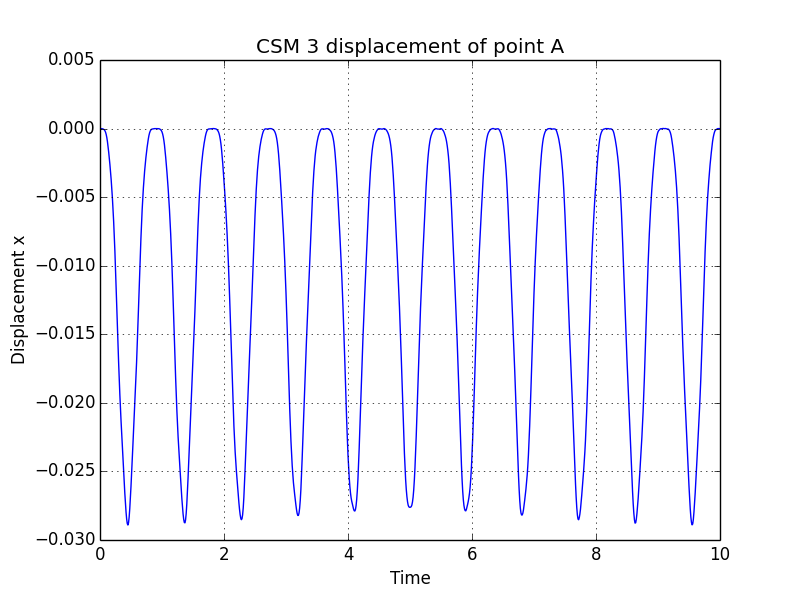
\includegraphics[width=0.75\linewidth]{./Verification_Validation//Hron_Turek/dis_x.png} 
    \caption{Displacement in x-direction} 
    \label{fig7:a} 
    \vspace{4ex}
  \end{subfigure}%% 
  \begin{subfigure}[b]{0.5\linewidth}
    \centering
    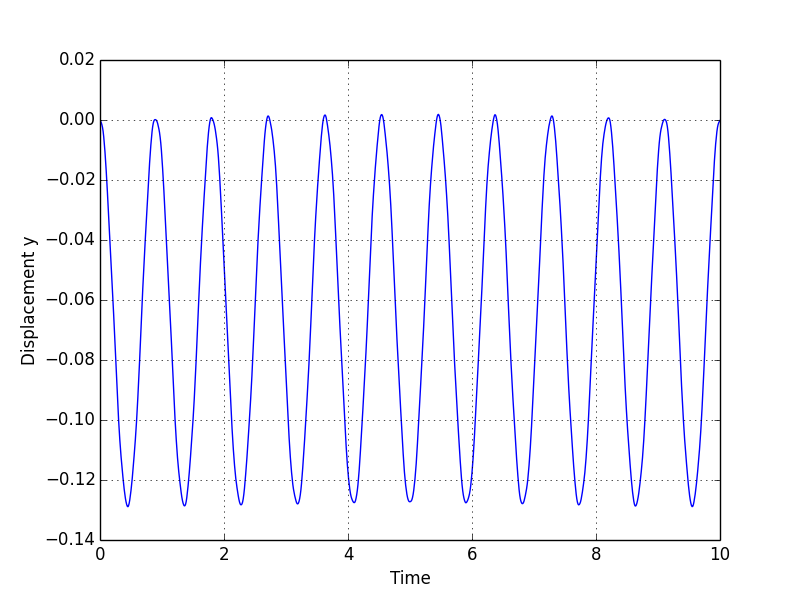
\includegraphics[width=0.75\linewidth]{./Verification_Validation//Hron_Turek/dis_y.png} 
    \caption{Displacement in x-direction} 
    \label{fig7:b} 
    \vspace{4ex}
  \end{subfigure} 
  \begin{subfigure}[b]{0.5\linewidth}
    \centering
    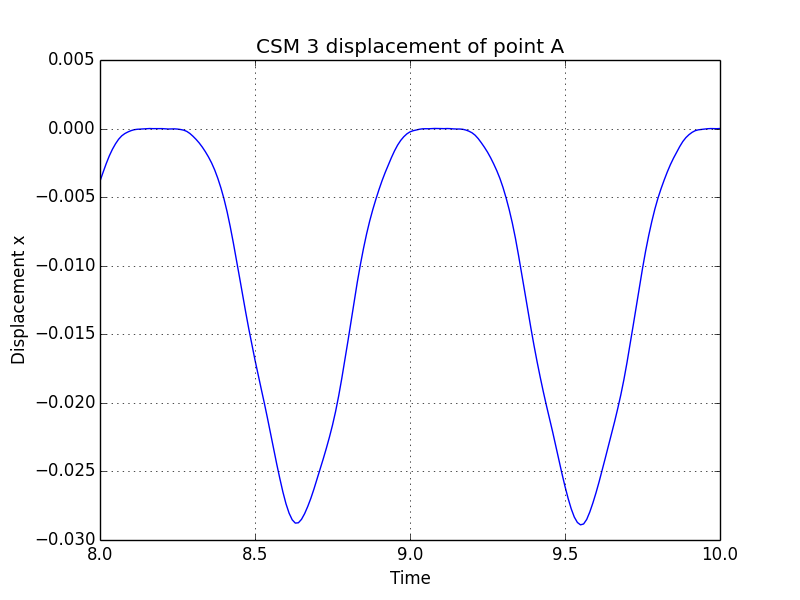
\includegraphics[width=0.75\linewidth]{./Verification_Validation//Hron_Turek/dis_x_short.png} 
    \caption{Displacement in x-direction} 
    \label{fig7:c} 
  \end{subfigure}%%
  \begin{subfigure}[b]{0.5\linewidth}
    \centering
    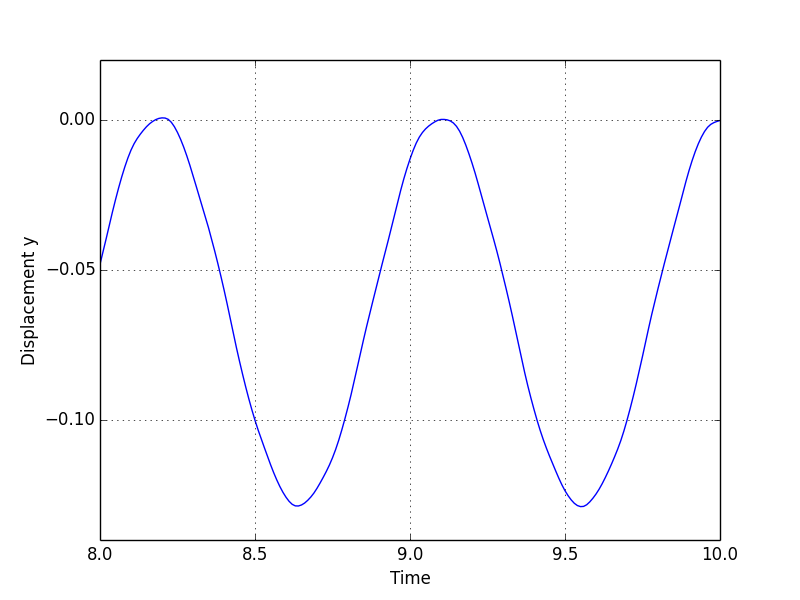
\includegraphics[width=0.75\linewidth]{./Verification_Validation/Hron_Turek/dis_y_short.png} 
    \caption{Displacement in x-direction} 
    \label{fig7:d} 
  \end{subfigure} 
  \caption{Displacement of point A}
  \label{fig7} 
\end{figure}


\subsection*{FSI test}
\begin{table}[ht]
\centering
\caption{FSI Parameters}
\label{my-label}
\begin{tabular}{|l|l|l|l|}
\hline
Parameters & FSI1 & FSI2 & FSI3 \\ \hline
$\rho_f[10^3 \frac{kg}{m^3}]$ & 1 & 1 & 1 \\ \hline
$\nu_f [10^{-3} \frac{m^2}{s}]$ & 1 & 1 & 1 \\ \hline
$u_0$ & 0.2 & 1 & 2 \\ \hline
Re = $\frac{U d}{\nu_f}$ & 20 & 100 & 200 \\ \hline
$\rho_s[10^3 \frac{kg}{m^3}]$ & 1 & 10 & 1 \\ \hline
$\nu_s$ & 0.4 & 0.4 & 0.4 \\ \hline
$\mu_s[10^6 \frac{m^2}{s}]$ & 0.5 & 0.5 & 2 \\ \hline
\end{tabular}
\end{table}
Results: 
\begin{table}[h]
\centering
\caption{FSI 1}
\label{my-label}
\begin{tabular}{|l|l|l|l|l|l|l|}
\hline
Cells & Dofs & ux of A $[x10^{-3}]$ & uy of A $[x10^{-3}]$ & Drag & Lift & Spaces \\ \hline
2698 & 7095 & 0.0234594 & 0.797218  & 14.4963 & 0.915801 & P1-P1-P1 stab= 0.01 \\ \hline
2698 & 23563 &0.0227418 &0.799314  &  14.1735 &0.761849 & P2-P2-P1 \\ \hline
10792 & 92992  &0.0227592 & 0.80795 & 14.1853 &  0.775063 &  P2-P2-P1 \\ \hline
43168 & 369448 & 00.227566 & 0.813184 & 14.2269 & 0.771071 & P2-P2-P1 \\ \hline
\textbf{ref} & \textbf{ref} & \textbf{0.0227} & \textbf{0.8209} & \textbf{14.295} & \textbf{0.7638} & \textbf{ref} \\ \hline
\end{tabular}
\end{table}



\newpage
OLD SHITZ FSI:
\begin{table}[h]
\centering
\caption{FSI 1}
\label{my-label}
\begin{tabular}{|l|l|l|l|l|l|l|}
\hline
Cells & Dofs & ux of A $[x10^{-3}]$ & uy of A $[x10^{-3}]$ & Drag & Lift & Spaces \\ \hline
2698 & 7095 & 0.0234594 & 0.797218  & 14.4963 & 0.915801 & P1-P1-P1 stab= 0.01 \\ \hline
2698 & 23563 & 0.02271 & 0.80288 & 14.1736 & 0.787891 & P2-P2-P1 \\ \hline
2698 & 23563 & 0.00581116 & 0.000000738678  & 12.07 & 0.02345 & P2-P2-P1 without weighting \\ \hline
10792 & 92992 & 0.0227341 & 0.808792 & 14.1855 & 0.801044 & P2-P2-P1 \\ \hline
43168 & 369448 & 0.227352 & 0.812595 & 14.227 & 0.797242 & P2-P2-P1 \\ \hline
\textbf{ref} & \textbf{ref} & \textbf{0.0227} & \textbf{0.8209} & \textbf{14.295} & \textbf{0.7638} & \textbf{ref} \\ \hline
\end{tabular}
\end{table}